 %!TEX root = ../dokumentation.tex

\chapter{Introduction}\label{cha:Introduction}

To introduce the content of this work the concepts of debugging and the behavior of shaders on the graphics pipeline are explained. After that the problem of debugging shaders in the graphics pipeline is shown and the objectives of this work are presented.

\section{Explanation of debugging}
\label{paragraph:debuging}

"Debugging is the process of locating and removing faults in computer programs" according to \myCite{Collins_debugging.2014}. The steps that are part of the debugging process are reproducing the problem, identifying the source of the problem and fixing the problem. All of these steps can be done manually but there are ways to improve and accelerate this process.

It is possible to write a program with formal verificattion. Here the program is based on a mathematical proof ensuring its correctness. For these programs debugging is not necessary but formal verification has its limits with porgrams getting too complex. \myCite{bolton2013using}

For debugging, to find problems there is the option of writing automated tests, inserting debug outputs on the console into the source code or writing states into log files. This enables the programmer to find anomalies before, while and after running the program.

When a way is found to reproduce the problem, to find the source of it the manual way is to increase the amount of debug outputs around the problematic part of the code and confine the point in the code at which the error occurs.

"Everyone knows that debugging is twice as hard as writing a program in the first place. So if you're as clever as you can be when you write it, how will you ever debug it?" according to \myCite{Kernighan.1982}. As this states, debugging is a quite exhausting and time consuming task. For that reason for most programming languages there are tools to aid the programmer to narrow down the source of the bug with following methods:

\begin{itemize}

\item Enabling the user to set breakpoints at which the program pauses and he can inspect the values of the variables directly within the code. By continuing the program to move to the next breakpoint or by going forward through the code step by step the point where the error occurs can be found. It is also possible to be able to add conditions to the breakpoints describing a state that has to be fulfilled for the debugger to pause. \myCite{Undo.2019}


\item Have the code throw an exception when unwanted behavior occurs and stop at this exception. By saving a stack of the calls which occurred before the exception was thrown or dumping the buffer, the programmer can retrace where the error may be found.\myCite{Jetbrains.2019}


\item Reverse debugging records all program activities and thereby it is possible to move backwards in addition to forward stepping from a set breakpoint and see the changes in the variables and the calls in the code leading to the problem.\myCite{Undo.2019}

\end{itemize}

When the source of the problem is found the final step of fixing the problem is to correct the code.

\section{Explanation of shaders in the graphics pipeline}

A shader is a program running on the GPU thereby mostly running as part of the graphics pipeline.\myCite{Khronos_shader.2019} The exception for this behavior is the compute shader which is independent from the graphics pipeline.\myCite{Khronos_compute.2019}

The main use of the graphics pipeline is to generate an graphical output in form of a raster image out of geometry data. The GPU is a hardware specialized for this process leading to improved performance implementing it compared to running the same calculations on the CPU. This is shown in more detail in the paragraph at the end of this section.

The most used types of shaders on the graphics pipeline are the vertex shader, the tesselation shader, the geometry shader and the fragment shader. Their basic functionality is described in the following paragraph showing the sequence of events within the graphics pipeline.

\paragraph{Structure of the graphics pipeline}
\label{paragraph:pipeline}

The graphics pipeline also known as rendering pipeline differentiates from framework to framework but the basic structure is identical.\myCite{Khronos_pipeline.2019} \myCite{Microsoft_pipeline.2018}

In the first stage the vertices are specified. The vertices are set up in an ordered list. By setting a primitive type it is determined how these vertices define the boundaries of primitives. Attributes are linked to the vertices adding data to them.

The second stage is the execution of the vertex shader for each defined vertex with its data. For each vertex the vertex shader generates an output vertex with data.

After the vertex stage multiple, optional stages can occur. Examples for these are the Tesselation stage or the Geometry stage where additional shaders are executed to implement additional changes to the vertices or even remove or add vertices.

In the following stage there are multiple optimization steps, the primitive assembly and the rasterization. The perspective divide and the viewport transformation are calculated. Through clipping, which is optional, primitives that overlap the edge of the viewing volume are split into multiple primitives and primitives outside the viewing volume are removed. Primitives are assembled according to the primitive type, so a list of primitives is constructed out of the list of vertices where each primitive is constructed out of multiple vertices. Face culling can occur as additional optimization removing primitives that face certain directions in the window space. The primitives are then rasterized into fragments within the raster of the render result. The data values linked to the vertices are set for each corresponding fregment by hardware based calculations.

Within the following fragment stage the fragment shader will be executed for each single fragment. The output data is calculated and attached to the corresponding fragment.

After the fragment stage the output of the render process is calculated. For each sample there are multiple optional filters that can be activated to change which fragments are used within this stage. Examples for these filters are the scissor test where a fragment is ignored when it's pixel lies outside of the rectangle of the screen or the depth test where the fragments order is changed when its depth fulfils specific, user defined conditions compared to another fragment's depth within the same sample. After all active filters were executed the color blending happens where the color between multiple fragments within the same sample is calculated together with a specific blending operation. The final data is written to the framebuffer.

The two most known uses of the graphics pipeline are within the graphics libraries OpenGL and Direct3D as shown in  \autoref{fig:pipeline_opengl} and \autoref{fig:pipeline_direct3d}

\begin{figure}[h!]
  \centering 
  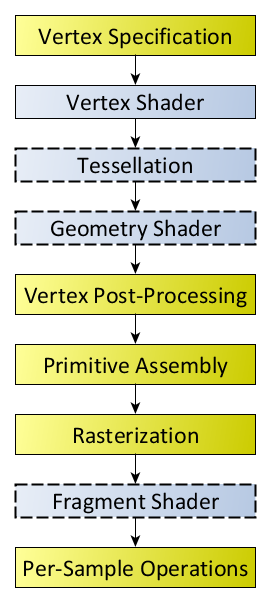
\includegraphics[scale=0.3]{Pipeline_OpenGL.png}
  \caption[Graphics pipeline by OpenGL \myCite{Khronos_pipeline.2019}]{Graphics pipeline by OpenGL}
  \label{fig:pipeline_opengl}
\end{figure}

\begin{figure}[h!]
  \centering 
  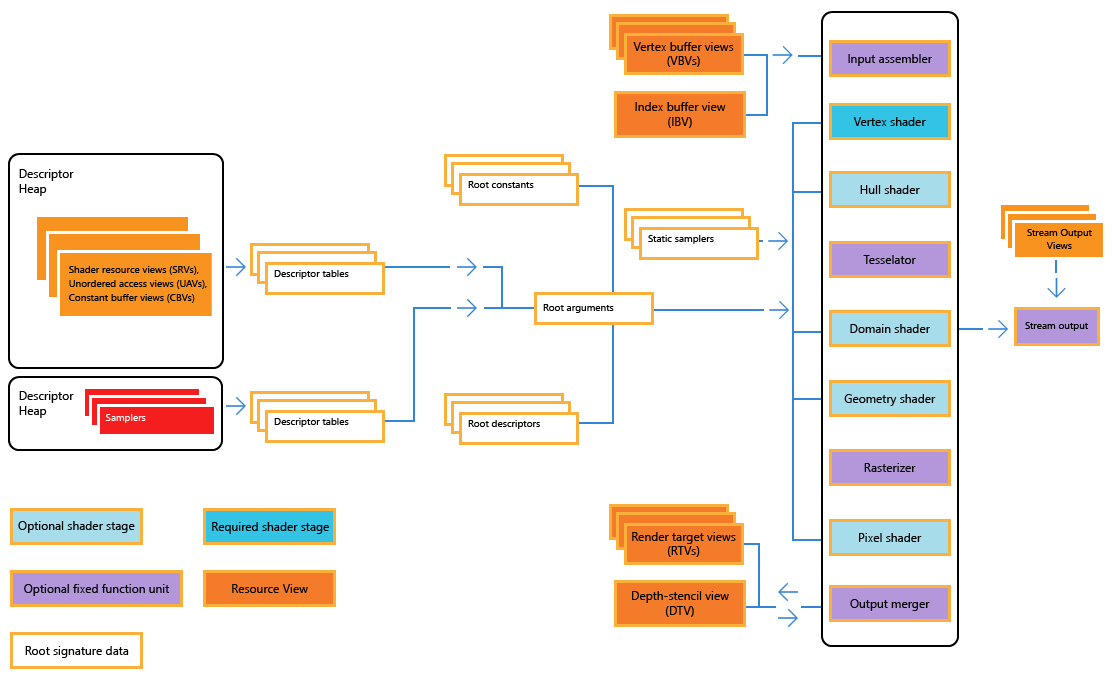
\includegraphics[scale=0.4]{Pipeline_Direct3D.png}
  \caption[Graphics pipeline by Direct3D \myCite{Microsoft_pipeline.2018}]{Graphics pipeline by Direct3D}
  \label{fig:pipeline_direct3d}
\end{figure}

\paragraph{Performance differences between graphics calculation on a GPU and a CPU}

The main advantage in using shaders in the graphics pipeline on the GPU lies in the increased performance compared to the CPU.
In this paragraph the performance differences between calculating graphics with the described graphics pipeline on a GPU and calculating it on a CPU will be demonstrated by showing an example.

The example is also implemented within the project created for this work.\myCite{project} The example consists of a simple triangle covering half the space of a window with 640 by 480 pixels as shown in \autoref{fig:triangleSample}. The example is run on a Nvidia GTX970 as GPU and a Intel i7-6700K as CPU. It has to be noted though that there are ways to further optimize the calculation on the CPU. For example the program is not multi threaded and is running in a JIT compiler. But it should be enough to serve as a rough example for the difference in performance.

Rendering the described image on the GPU takes about 0.0015 ms while calculating the same output in the CPU with the implemented example takes about 800 ms. The rasterizing step with calculating the data for all fragment from the data of the vertices within the corresponding primitives alone takes over 300 ms in this example.

As shown with this example it is desirable to use the graphics pipeline supported on the GPU.

\begin{figure}[h!]
  \centering 
  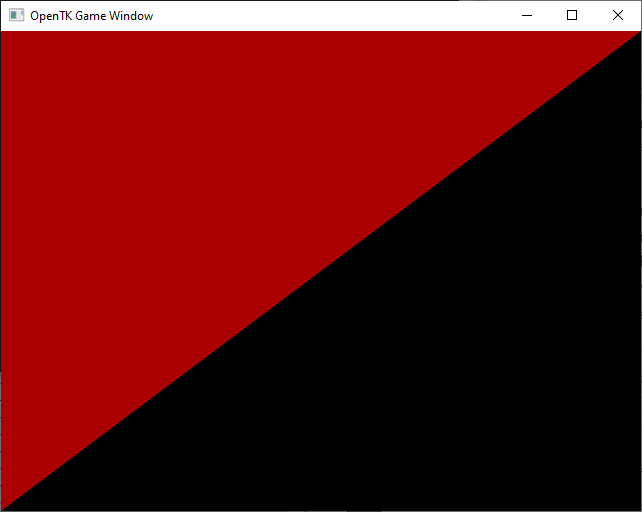
\includegraphics[scale=0.5]{triangleExample.png}
  \caption[Screenshot of triangle test render]{Example of a triangle rendered on a window with 640 by 480 pixels}
  \label{fig:triangleSample}
\end{figure}

\section{Problem with debugging shaders in the graphics pipeline}
\label{section:problems}

As established before there are advantages in the use of shaders and the GPU. There are different tools to support with the implementation of shaders.\myCite{Jones.2019}\myCite{scherzer_visualstudio.2019}\myCite{scherzer_npp.2019} For debugging shaders on the graphics pipeline though there are no general solutions that aid the user in the process.

While most CPUs are very broad in their functionality and support debugging by itself a GPU is more specialized in the way it functions and usually does not have the option to pause the code to enable inspections at runtime and does not even have access to a console or logger to write states into.\myCite{Fox.2017}

As explained in more detail in \autoref{section:debuggingMethods_drivers} it is possible to enable debugging on the GPU with specialized drivers for specific hardware.\myCite{Nvidia_debug.2019}\myCite{Microsoft_debug.2016}

There are also approaches which enable debugging of compute shader code by translating it from another language. The code is written in a language for the CPU which supports debugging with tools. It is run and debugged on the CPU while it is translated to the shader language to run as a compute shader on the GPU.
See more in \autoref{section:computeApproaches}.

\section{Objective of creating a general solution for debugging shaders in the graphics pipeline}
\label{paragraph:objective}

The objective of this work is to create a general solution to enable debugging of shaders within the graphics pipeline. The goals this solution should fulfill are the following:

\begin{itemize}
	\item Different methods to assist the programmer in debugging as shown in \autoref{paragraph:debuging} are usable.
	\item The solution is not dependent on the use of specific graphics cards or drivers.
	\item It is possible to switch between a mode where debugging is enabled and a mode where the shaders run as usual, so the program can run with the full performance and without interference of the debugger.
	\item The resulting output per render iteration of the debugger is close to the output of the program with the undebugged shader. It is close enough that the programmer can see what the rendering result without the debugger would look like. Errors like those resulting from the use of float variables with their inaccuracies are tolerable because there are tolerances within human perception where minimal changes in position or color within a rendered result do not matter.\myCite{Franz.2006}
	\item Performance is not a major requirement while running the debugger. It is possible to see the output and the values of the shader within each frame and iterate through the frames. It is not necessary to view the result in the speed of the final application while debugging. In existing debugging tools the programmer also has to wait until the functionality of the program reaches the point where the part of the program wished to debug is executed. This means the debugger does not have to be as fast as a user interface with the goal of a fluid user experience would have to, but it suffices to have the user to not wait too long. According to \myCite{Nielson.1993} there are the following three important limits:
	\begin{itemize}
	\item "0.1 second is about the limit for having the user feel that the system is reacting instantaneously, meaning that no special feedback is necessary except to display the result."
	\item "1.0 second is about the limit for the user's flow of thought to stay uninterrupted, even though the user will notice the delay. Normally, no special feedback is necessary during delays of more than 0.1 but less than 1.0 second, but the user does lose the feeling of operating directly on the data."
    \item "10 seconds is about the limit for keeping the user's attention focused on the dialogue. For longer delays, users will want to perform other tasks while waiting for the computer to finish, so they should be given feedback indicating when the computer expects to be done. Feedback during the delay is especially important if the response time is likely to be highly variable, since users will then not know what to expect."
	\end{itemize}
	Therefor the targeted performance for the user not having to wait to long should eneble the user to reach a debugging point within maximum 10 seconds.
\end{itemize}




